\documentclass[journal,12pt,twocolumn]{IEEEtran}

\usepackage{setspace}
\usepackage{gensymb}

\singlespacing


\usepackage[cmex10]{amsmath}

\usepackage{amsthm}

\usepackage{mathrsfs}
\usepackage{txfonts}
\usepackage{stfloats}
\usepackage{bm}
\usepackage{cite}
\usepackage{cases}
\usepackage{subfig}

\usepackage{longtable}
\usepackage{multirow}

\usepackage{enumitem}
\usepackage{mathtools}
\usepackage{steinmetz}
\usepackage{tikz}
\usepackage{circuitikz}
\usepackage{verbatim}
\usepackage{tfrupee}
\usepackage[breaklinks=true]{hyperref}
\usepackage{graphicx}
\usepackage{tkz-euclide}
\usepackage{float}

\usetikzlibrary{calc,math}
\usepackage{listings}
    \usepackage{color}                                            %%
    \usepackage{array}                                            %%
    \usepackage{longtable}                                        %%
    \usepackage{calc}                                             %%
    \usepackage{multirow}                                         %%
    \usepackage{hhline}                                           %%
    \usepackage{ifthen}                                           %%
    \usepackage{lscape}     
\usepackage{multicol}
\usepackage{chngcntr}

\DeclareMathOperator*{\Res}{Res}

\renewcommand\thesection{\arabic{section}}
\renewcommand\thesubsection{\thesection.\arabic{subsection}}
\renewcommand\thesubsubsection{\thesubsection.\arabic{subsubsection}}

\renewcommand\thesectiondis{\arabic{section}}
\renewcommand\thesubsectiondis{\thesectiondis.\arabic{subsection}}
\renewcommand\thesubsubsectiondis{\thesubsectiondis.\arabic{subsubsection}}


\hyphenation{op-tical net-works semi-conduc-tor}
\def\inputGnumericTable{}                                 %%

\lstset{
%language=C,
frame=single, 
breaklines=true,
columns=fullflexible
}
\begin{document}
\newtheorem{theorem}{Theorem}[section]
\newtheorem{problem}{Problem}
\newtheorem{proposition}{Proposition}[section]
\newtheorem{lemma}{Lemma}[section]
\newtheorem{corollary}[theorem]{Corollary}
\newtheorem{example}{Example}[section]
\newtheorem{definition}[problem]{Definition}

\newcommand{\BEQA}{\begin{eqnarray}}
\newcommand{\EEQA}{\end{eqnarray}}
\newcommand{\define}{\stackrel{\triangle}{=}}
\bibliographystyle{IEEEtran}
\providecommand{\mbf}{\mathbf}
\providecommand{\pr}[1]{\ensuremath{\Pr\left(#1\right)}}
\providecommand{\qfunc}[1]{\ensuremath{Q\left(#1\right)}}
\providecommand{\sbrak}[1]{\ensuremath{{}\left[#1\right]}}
\providecommand{\lsbrak}[1]{\ensuremath{{}\left[#1\right.}}
\providecommand{\rsbrak}[1]{\ensuremath{{}\left.#1\right]}}
\providecommand{\brak}[1]{\ensuremath{\left(#1\right)}}
\providecommand{\lbrak}[1]{\ensuremath{\left(#1\right.}}
\providecommand{\rbrak}[1]{\ensuremath{\left.#1\right)}}
\providecommand{\cbrak}[1]{\ensuremath{\left\{#1\right\}}}
\providecommand{\lcbrak}[1]{\ensuremath{\left\{#1\right.}}
\providecommand{\rcbrak}[1]{\ensuremath{\left.#1\right\}}}
\theoremstyle{remark}
\newtheorem{rem}{Remark}
\newcommand{\sgn}{\mathop{\mathrm{sgn}}}
\providecommand{\abs}[1]{\vert#1\vert}
\providecommand{\res}[1]{\Res\displaylimits_{#1}} 
\providecommand{\norm}[1]{\lVert#1\rVert}
%\providecommand{\norm}[1]{\lVert#1\rVert}
\providecommand{\mtx}[1]{\mathbf{#1}}
\providecommand{\mean}[1]{E[ #1 ]}
\providecommand{\fourier}{\overset{\mathcal{F}}{ \rightleftharpoons}}
%\providecommand{\hilbert}{\overset{\mathcal{H}}{ \rightleftharpoons}}
\providecommand{\system}{\overset{\mathcal{H}}{ \longleftrightarrow}}
	%\newcommand{\solution}[2]{\textbf{Solution:}{#1}}
\newcommand{\solution}{\noindent \textbf{Solution: }}
\newcommand{\cosec}{\,\text{cosec}\,}
\providecommand{\dec}[2]{\ensuremath{\overset{#1}{\underset{#2}{\gtrless}}}}
\newcommand{\myvec}[1]{\ensuremath{\begin{pmatrix}#1\end{pmatrix}}}
\newcommand{\mydet}[1]{\ensuremath{\begin{vmatrix}#1\end{vmatrix}}}
\numberwithin{equation}{subsection}
\makeatletter
\@addtoreset{figure}{problem}
\makeatother
\let\StandardTheFigure\thefigure
\let\vec\mathbf
\renewcommand{\thefigure}{\theproblem}
\def\putbox#1#2#3{\makebox[0in][l]{\makebox[#1][l]{}\raisebox{\baselineskip}[0in][0in]{\raisebox{#2}[0in][0in]{#3}}}}
     \def\rightbox#1{\makebox[0in][r]{#1}}
     \def\centbox#1{\makebox[0in]{#1}}
     \def\topbox#1{\raisebox{-\baselineskip}[0in][0in]{#1}}
     \def\midbox#1{\raisebox{-0.5\baselineskip}[0in][0in]{#1}}
\vspace{3cm}
\title{GATE ASSIGNMENT 1}
\author{Amulya Tallamraju \\ AI20BTECH11003}
\maketitle
\newpage
\bigskip
\renewcommand{\thefigure}{\theenumi}
\renewcommand{\thetable}{\theenumi}
Download all python codes from 
\begin{lstlisting}
https://github.com/AmulyaTallamraju/EE3900/blob/main/GATE_Assignment-1/codes/GATE_Assignment-1.py
\end{lstlisting}
%
and latex-tikz codes from 
%
\begin{lstlisting}
https://github.com/AmulyaTallamraju/EE3900/blob/main/GATE_Assignment-1/GATE_Assignment-1.tex
\end{lstlisting}
%
\section{GATE EC 2021 Q.41}
Consider  the  signals  $x[n]=2^{n-1}u[-n+2]$ and $y[n]=2^{-n+2}u[n+1]$, 
where $u[n]$ is the unit step sequence. Let $X(e^{j\omega})$ and $Y(e^{j\omega})$ the discrete-time  Fourier  transform  of  $x[n]$  and  $y[n]$,  respectively.  The  value  of  the 
integral 
\begin{align}
    \frac{1}{2\pi} \int_{0}^{2\pi} X(e^{j\omega}) Y(e^{-j\omega}) \, d\omega
\end{align}
is
%
\section{Solution}
\begin{theorem}[Convolution Theorem] \label{ct}
Let $f$ and $g$ be two functions with convolution $f*g$. Let $F$ be the Fourier transform operator. Then
\begin{align}
F(f * g)=F(f) \cdot F(g)\\
F(f \cdot g)=F(f) * F(g)
\end{align}
\end{theorem}
If the DTFT of $y[n]$ is $Y(e^{j\omega})$  then using the time reversal property, the DTFT of $y[-n]$ is 
\begin{align}
Y\brak{\frac{1}{e^{j\omega}}}=Y(e^{-j\omega})  
\end{align}
Let 
\begin{align} \label{convolu}
    z[n]=x[n]*y[-n]
\end{align}
Let $Z(e^{j\omega})$ be the DTFT of $z[n]$. Using Theorem \ref{ct} we get
\begin{align}
  Z(e^{j\omega})= X(e^{j\omega}) Y(e^{-j\omega}) 
\end{align}
By applying IDTFT, we can write:
\begin{align}
z[n]=\frac{1}{2\pi} \int_{0}^{2\pi} X(e^{j\omega}) Y(e^{-j\omega}) e^{j\omega n}\, d\omega  
\end{align}
Putting $n=0$, we get the required value which is
\begin{align}
z[0]=\frac{1}{2\pi} \int_{0}^{2\pi} X(e^{j\omega}) Y(e^{-j\omega})\, d\omega 
\end{align}
The $\mathcal{Z}$ transform for a sequence of the form $a^{(n)}u[n]$ when $d=n$ is given by
\begin{align}\label{Z1}
\sum _{n=-\infty }^{\infty }\brak{{az^{-1}}}^n u[n]
=\brak{({1-az^{-1}})^{-1}}
\end{align}
provided, $\abs{z}<\abs{a}$, when $n<0$ or  $\abs{a}<\abs{z}$, when $n>0$ which is the region of convergence.
From \eqref{Z1}, $\mathcal{Z} $ transform of $x[n]$ in the Region of Convergence is
\begin{align}
    X(z)&={\mathcal {Z}}\{x[n]\}
    =\frac{1}{2}\brak{{\brak{2z^{-1}}^2}\brak{1-\frac{z}{2}}^{-1}}
\end{align}
From \eqref{Z1} $\mathcal{Z} $ transform of $y[n]$ in the Region of Convergence is
\begin{align}
    Y(z)&={\mathcal {Z}}\{y[n]\}=4\brak{{2z}\brak{1-\frac{z^{-1}}{2}}^{-1}}
\end{align}
Now,
\begin{align}\label{aa}
  Z(z)&= X(z) Y\brak{\frac{1}{z}} \\
  &=2\brak{ {\brak{2z^{-1}}^3} {\brak{1-\frac{z}{2}}^{-2}}}
\end{align}
The DTFT of $x[n]$ converges for all values of $\omega$ since,
\begin{align}
    z=e^{j\omega}\\
    a=2\\
    \abs{{z}{a}}=\frac{1}{2}
\end{align}
The DTFT of $y[n]$ also converges for all values of $\omega$ since 
\begin{align}
    z=e^{j\omega}\\
    a=\frac{1}{2}\\
    \abs{az^{-1}}=\frac{1}{2}
\end{align}
\begin{align}
\sum _{n=-\infty }^{\infty}\brak{az^{-1}}^nu[-n]
&=\sum _{n=-\infty }^{\infty }\brak{az^{-1}}^{-n}u[n]\\
&=\sum _{n=0 }^{\infty }\brak{\frac{z}{a}}^n\\
&=\brak{\brak{1-\frac{z}{a}}^{-1}}
\end{align}
Differentiating the above expression 
\begin{align}
&\sum _{n=-\infty }^{\infty }na^{-n}z^{n-1}u[n]
=\frac{1}{a}\brak{\brak{1-\frac{z}{a}}^{-2}}\\
\implies & \sum _{n=-\infty }^{\infty }na^{-n}z^{n-4}u[n]
=\frac{1}{a}\brak{z^{-3}\brak{1-\frac{z}{a}}^{-2}}\\
\implies & \sum _{n=-\infty }^{\infty }na^{-n+5}z^{n-4}u[n]
=a^4\brak{z^{-3}\brak{1-\frac{z}{a}}^{-2}}\\
\implies & \sum _{n=-\infty }^{\infty }(4-n)a^{n+1}z^{-n}u[4-n]=a^4\brak{z^{-3}\brak{1-\frac{z}{a}}^{-2}}
\end{align}
Comparing the above equation with \eqref{aa} we get
$a=2$.
From the definition of DTFT we have
\begin{align}
 Z(z=e^{j\omega})&=  \sum _{n=-\infty }^{\infty }z[n]z^{-n}\label{2}
\end{align}
Thus
\begin{align}
 z[n]=(4-n)2^{n+1}u[4-n]
\end{align}
\begin{align}
    \therefore \frac{1}{2\pi} \int_{0}^{2\pi} X(e^{j\omega}) Y(e^{-j\omega}) \, d\omega =z[0]=8
\end{align}
\begin{figure}[!h]
         \centering
         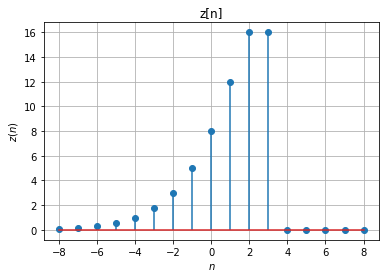
\includegraphics[width=\columnwidth]{z[n].png}
         \caption{Plot of z[n]}
         \label{plot}
\end{figure}
\end{document}
